\documentclass{beamer}
\usepackage{relsize}
\usepackage{color}

\usepackage{listings}
\usetheme{CambridgeUS}
%\usepackage{beamerthemesplit} % new
\usepackage{enumitem}
\usepackage{amsmath}                    % See geometry.pdf to learn the layout options.
\usepackage{amsthm}                   % See geometry.pdf to learn the layout options. There
\usepackage{amssymb}                    % See geometry.pdf to learn the layout options.
\usepackage[utf8]{inputenc}
\usepackage{graphicx}
\usepackage[english,bulgarian]{babel}

\usepackage{caption}
\usepackage{tikz}
\usetikzlibrary{shapes,arrows,positioning,calc,positioning,fit,chains}

\usetheme{CambridgeUS}
\usecolortheme{crane}

\lstset{language=C++,
                basicstyle=\ttfamily,
                keywordstyle=\color{blue}\ttfamily,
                stringstyle=\color{red}\ttfamily,
                commentstyle=\color{green}\ttfamily,
                morecomment=[l][\color{magenta}]{\#}
}

\tikzset{
block/.style = {draw, fill=white, rectangle,align = center},
entry/.style = {draw, fill=black, circle, radius=3em},
condition/.style = {draw, fill=white, diamond, align = center,node distance=3cm},
fork/.style = {draw, fill=black, circle,inner sep=1pt},
lnode/.style={rectangle split, rectangle split parts=3,draw, rectangle split horizontal},
treenode/.style = {align=center, inner sep=0pt, text centered, circle, font=\sffamily\bfseries, draw=black, fill=white, text width=1.5em},
flexnode/.style = {align=center, text centered, ellipse, font=\sffamily\bfseries, draw=black, fill=white},
token/.style={rectangle split, rectangle split parts=2,draw, rectangle split horizontal=false}
}


\newtheorem{mydef}{Дефиниция}[section]
\newtheorem{lem}{Лема}[section]
\newtheorem{thm}{Твърдение}[section]

\DeclareMathOperator{\restrict}{\upharpoonright}

\setitemize{label=\usebeamerfont*{itemize item}%
  \usebeamercolor[fg]{itemize item}
  \usebeamertemplate{itemize item}}

\setbeamercovered{transparent}

\captionsetup{font=tiny} 

\begin{document}
\title[Дървета]{Двоични дървета}
\frame{\titlepage}

\section{Двоични дървета}
\subsection{}

\begin{frame}[fragile]
\frametitle{Фамилно дърво}


\begin{columns}[t]
  \begin{column}{0.3\textwidth}

    \begin{itemize}
      \item родител, наследник
      \item корен
      \item листо
      \item път
      \item ниво
    \end{itemize}

  \end{column}
  \begin{column}{0.7\textwidth}

\begin{figure}
  \centering
  \begin{tikzpicture}[auto, level 1/.style={sibling distance=4cm},level 2/.style={sibling distance=3cm},>=latex',edge from parent/.style={draw,-latex}]
  \node [] {баща}
    child {
      node [] {син 1}
      child {
        node [] {внук 1}
      }
      child {
        node [] {внук 2}
      }
    }
    child {
      node [] {син 2}
      child {
        node [xshift=1cm] {внук 3}
        child {
          node [xshift=-1cm] {правнук 1}
        }
      }
    };
  \end{tikzpicture}
\end{figure}
  \end{column}
\end{columns}

\end{frame}


\begin{frame}[fragile]
  \frametitle{Дефиниции}
  
      \begin{itemize}
        \item Свързан неориентиран граф без цикли
      \end{itemize}
  
      \vspace{1.5em}
       Индуктивна дефиниция
  
  \begin{columns}[t]
    \begin{column}{0.65\textwidth}
  
  
      \begin{itemize}
        \item Фиксираме елемент $() \notin D$ и го наричаме \emph{``празно дърво''}
        \item Празното дърво е дърво
        \item Ако $L_T$ и $R_T$ са дървета, а $x$ е елемент ($x \in D$), то \emph{тройката (структурата)} $T=(x,L_T,R_T)$ наричаме двоично дърво $T$ с \emph{корен} $x$, ляво поддърво $L_T$ и дясно поддърво $R_T$.
      \end{itemize}
  
    \end{column}
    \begin{column}{0.35\textwidth}
  
      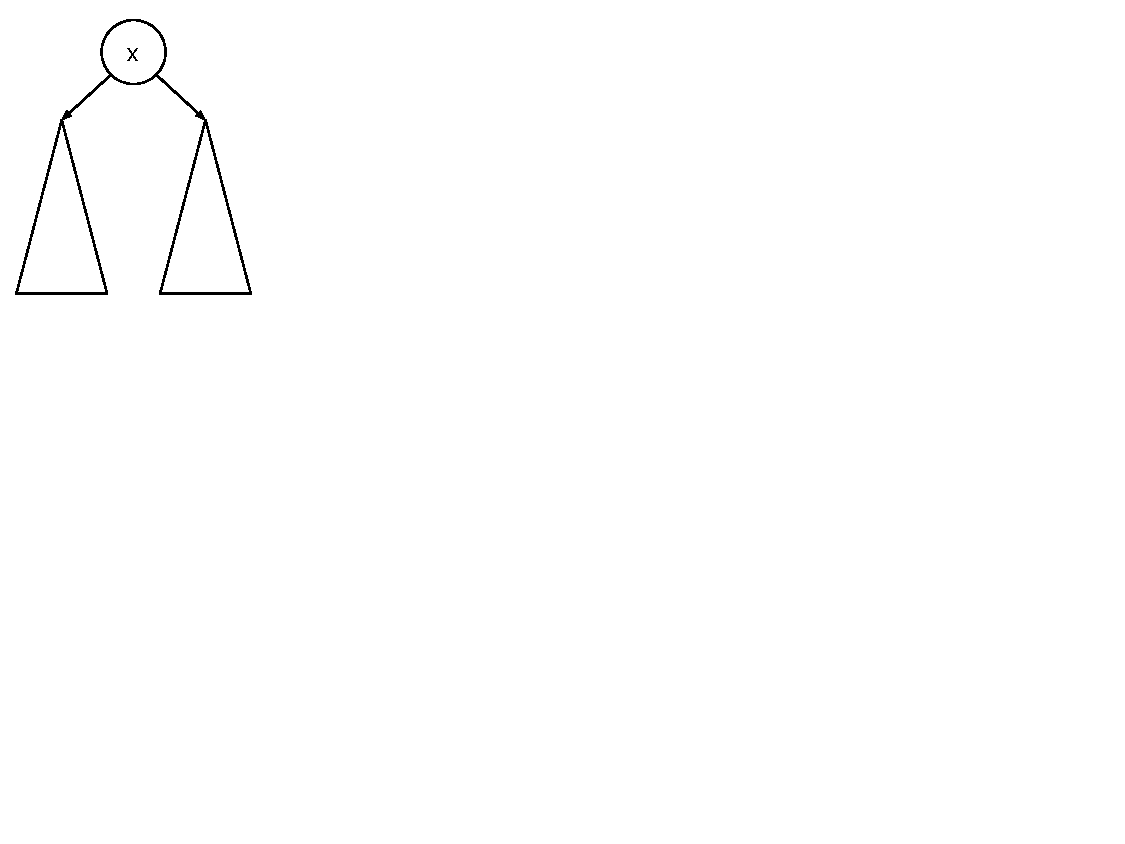
\includegraphics[width=9cm]{images/tree_recursive}
  
    \end{column}
  \end{columns}
    
  \end{frame}
  

\begin{frame}[fragile]
\frametitle{Дърво с числа}


    \begin{lstlisting}[basicstyle=\small,language=Haskell]
data IntTree = Empty | Node IntTree IntTree
    \end{lstlisting}

    
    \begin{columns}[t]
      \begin{column}{0.3\textwidth}

        \begin{lstlisting}[basicstyle=\tiny,language=Haskell]
mytree = 
  Node 7
      (Node 30 
            (Node 15 Empty Empty)
            (Node 3 Empty Empty))
      (Node 77
            Empty
            (Node 15
                  (Node 70 Empty Empty)
                  Empty))
        \end{lstlisting}
              
      \end{column}
      \begin{column}{0.7\textwidth}
        \begin{figure}
          \centering
          \begin{tikzpicture}[auto, level 1/.style={sibling distance=2cm},level 2/.style={sibling distance=2cm},>=latex',edge from parent/.style={draw,-latex}]
          \node [] {7}
            child {
              node [] {30} 
              child {
                node [] {15}
              }
              child {
                node [] {3} 
              }
            }
            child {
              node [] {77}
              child {
                node [xshift=1cm] {15}
                child {
                  node [xshift=-1cm] {70}
                }
              }
            };
          \end{tikzpicture}
        \end{figure}    
        
      \end{column}
    \end{columns}
    
    


\end{frame}


\section{Операции}
\begin{frame}
\centerline{Операции}
\end{frame}

\begin{frame}[fragile]
  \frametitle{Позиция на елемент}
      
  \begin{columns}[t]
    \begin{column}{0.3\textwidth}
  
      \begin{itemize}
        \item Търсене
        \item Вмъкване
        \item Промяна
        \item Изтриване
      \end{itemize}

    \end{column}
    \begin{column}{0.7\textwidth}
      \begin{figure}
        \centering
        \begin{tikzpicture}[auto, level 1/.style={sibling distance=2cm},level 2/.style={sibling distance=2cm},>=latex',edge from parent/.style={draw,-latex}]
        \node [] {7}
          child {
            node [] {30} 
            child {
              node [] {15}
            }
            child {
                node [] {3} 
                  child {
                  node [xshift=-1cm] {}
                  edge from parent[draw,dashed,text=red] node[left] {L}
                  }
              edge from parent[text=red] node[right] {R}
            }
            edge from parent[text=red] node[left] {L}
          }
          child {
            node [] {77}
            child {
              node [xshift=1cm] {15}
              child {
                node [xshift=-1cm] {70}
              }
            }
          };
        \end{tikzpicture}
      \end{figure}
  
    \end{column}
  \end{columns}
  
  \end{frame}
  
  \begin{frame}[fragile]
    \frametitle{Проверка за принадлежност}
    
        \begin{itemize}
          \item Среща ли се елементът $y$ сред елементите на дървото $T$?
        \end{itemize}
    
    
    \begin{columns}[t]
      \begin{column}{0.65\textwidth}
    
        \begin{flushleft}
        \relscale{0.5}
        \begin{itemize}
          \item Празното дърво е дърво
          \item Ако $L_T$ и $R_T$ са дървета, а $x$ е елемент ($x \in D$), то \emph{тройката (структурата)} $T=(x,L_T,R_T)$ наричаме двоично дърво $T$ с \emph{корен} $x$, ляво поддърво $L_T$ и дясно поддърво $R_T$.
        \end{itemize}
        \end{flushleft}
    
      \end{column}
      \begin{column}{0.35\textwidth}
    
        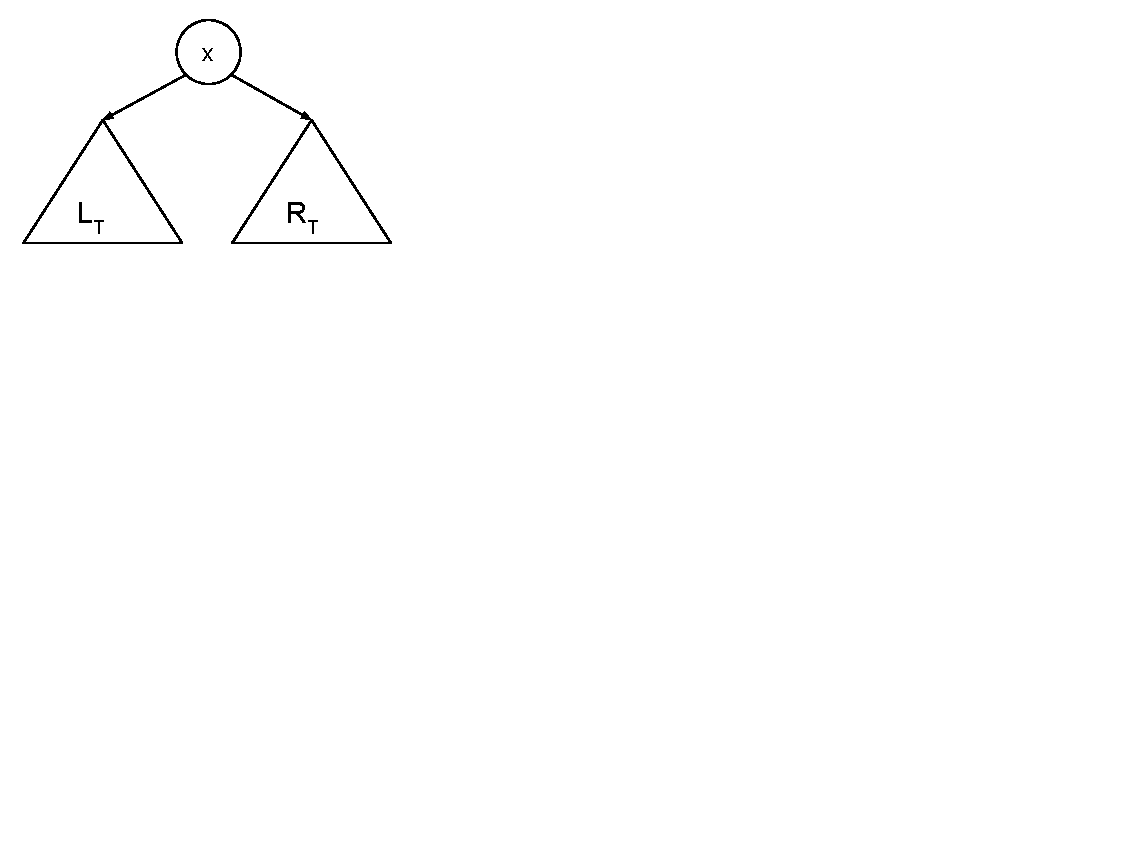
\includegraphics[width=8cm]{images/tree_recursive_op_2}
    
      \end{column}
    \end{columns}
    
    \vspace{-100px}
    
     \texttt{bool member (int y, T):}
    
        \begin{itemize}
          \item Ако дървото е празно, то $y$ не е елемент на дървото. \texttt{return false}
          \item  Ако $T=(x,L_T,R_T)$ е непразно, то $y$ е елемент на $T$, ако $y==x$ или $y$ е елемент на $L_T$ или $y$ е елемент на $R_T$.
          \item \texttt{return y==root(t) || member (y, LT) || member (y,RT)}
        \end{itemize}
    
    \end{frame}
    
    
    
    
    
    \begin{frame}[fragile]
    \frametitle{Сума на елементите}
    
        \begin{itemize}
          \item Каква е сумата на елементите на дървото?
        \end{itemize}
    
    
    \begin{columns}[t]
      \begin{column}{0.65\textwidth}
    
        \begin{flushleft}
        \relscale{0.5}
        \begin{itemize}
          \item Празното дърво е дърво
          \item Ако $L_T$ и $R_T$ са дървета, а $x$ е елемент ($x \in D$), то \emph{тройката (структурата)} $T=(x,L_T,R_T)$ наричаме двоично дърво $T$ с \emph{корен} $x$, ляво поддърво $L_T$ и дясно поддърво $R_T$.
        \end{itemize}
        \end{flushleft}
    
      \end{column}
      \begin{column}{0.35\textwidth}
    
        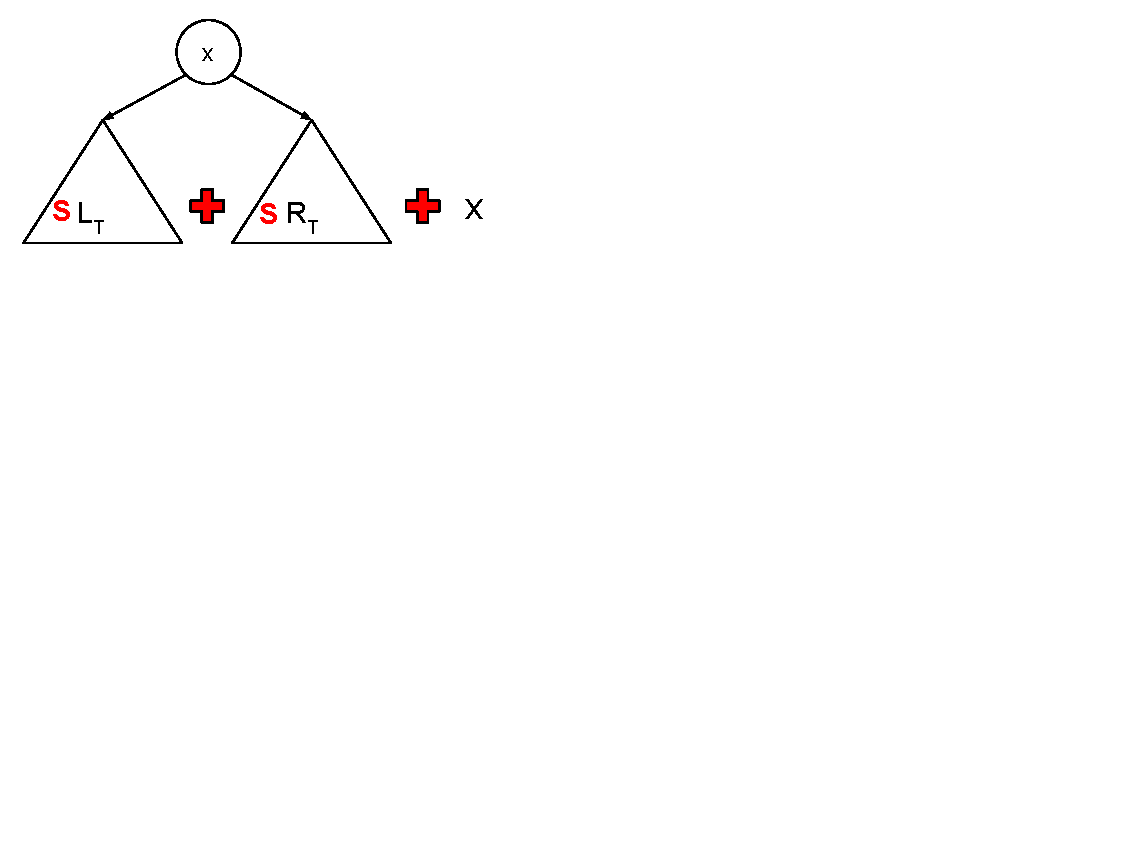
\includegraphics[width=8cm]{images/tree_recursive_op_sum}
    
      \end{column}
    \end{columns}
    
    \vspace{-100px}
    
     \texttt{int sum (T):}
    
        \begin{itemize}
          \item Ако дървото е празно, то сумата на елементите е $0$. \texttt{return 0}
          \item  Ако $T=(x,L_T,R_T)$ е непразно, то сумата на елементите е сбора на сумата на елементите на $L_T$, на сумата на елементите на $R_T$ и на числото $x$.
          \item \texttt{return root(t) + sum (LT) + sum (RT)}
        \end{itemize}
    
    \end{frame}
    
    
    
    \begin{frame}[fragile]
    \frametitle{Други прости рекурсивни операции}
    
        \begin{itemize}
          \item Най-голям елемент в дървото
          \item Брой на елементитите в дървото
          \item Височина на дървото
          \item Брой на листата в дървото
        \end{itemize}
    
    
    \begin{columns}[t]
      \begin{column}{0.65\textwidth}
    
        \begin{flushleft}
        \relscale{0.5}
        \begin{itemize}
          \item Празното дърво е дърво
          \item Ако $L_T$ и $R_T$ са дървета, а $x$ е елемент ($x \in D$), то \emph{тройката (структурата)} $T=(x,L_T,R_T)$ наричаме двоично дърво $T$ с \emph{корен} $x$, ляво поддърво $L_T$ и дясно поддърво $R_T$.
        \end{itemize}
        \end{flushleft}
    
      \end{column}
      \begin{column}{0.35\textwidth}
    
        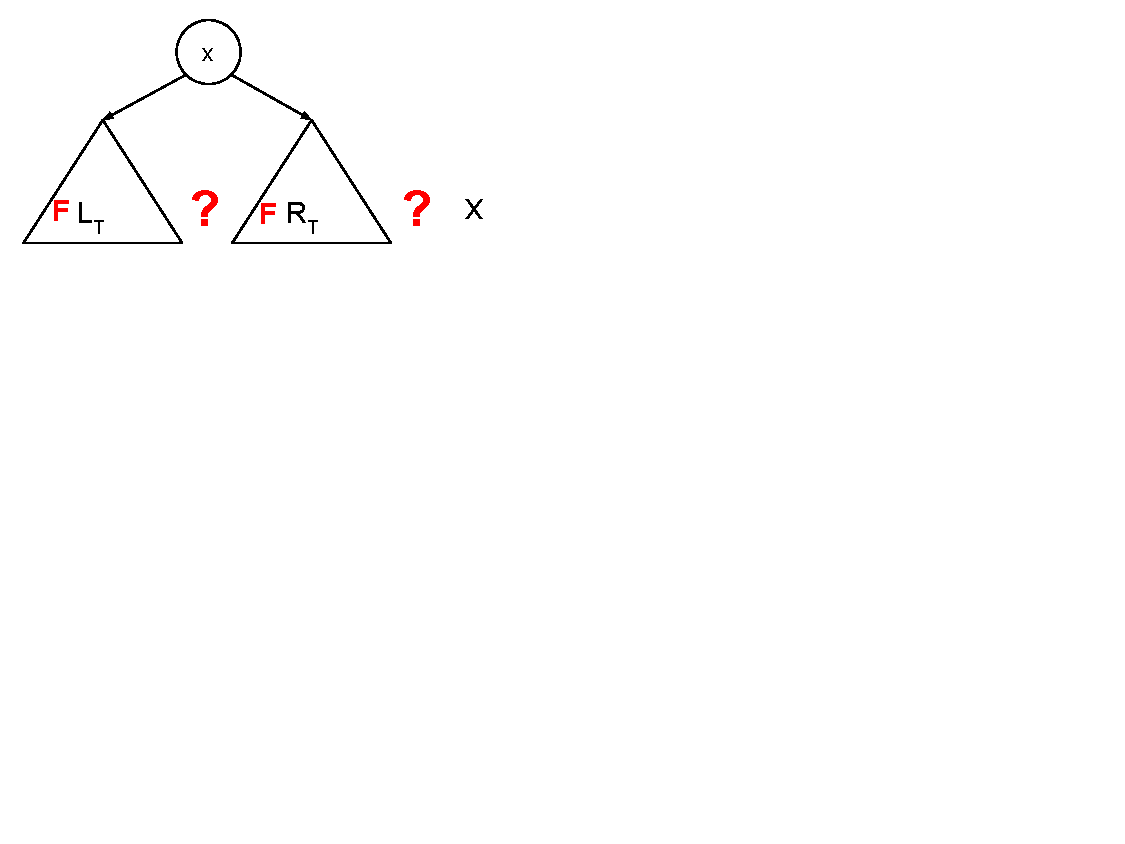
\includegraphics[width=8cm]{images/tree_recursive_op_qm}
    
      \end{column}
    \end{columns}
    \end{frame}
        

\begin{frame}
  \centerline{Сериализация и десериализация}
\end{frame}

\begin{frame}[fragile]
  \frametitle{Scheme формат}


\begin{itemize}
  \item Пазно дърво: $()$
  \item Дърво с корен $x$, ляво поддърво $l$ и дясно поддърво $r$: $(x\: l \: r)$
\end{itemize}

\bigskip

\begin{columns}[t]
  \begin{column}{0.35\textwidth}

\begin{verbatim}
(7 
  (30 
      (15 () ()) 
      (3 () ())) 
  (77 
      () 
      (15 
          (70 () ()) 
          ())))  
\end{verbatim}
    
  \end{column}
  \begin{column}{0.65\textwidth}
\begin{verbatim}
Node 7
  (Node 30 
        (Node 15 Empty Empty)
        (Node 3 Empty Empty))
  (Node 77
        Empty
        (Node 15
              (Node 70 Empty Empty)
              Empty))
\end{verbatim}
  \end{column}
\end{columns}




\end{frame}

\section{Двоични наредени дървета}
\begin{frame}
  \centerline{Двоични наредени дървета}
\end{frame}



\begin{frame}[fragile]
  \frametitle{Двоично наредено дърво}
      
  \begin{columns}[t]
    \begin{column}{0.3\textwidth}
  
      \begin{itemize}
        \item Търсене
        \item Минимален и максимален елемент
        \item Вмъкване
      \end{itemize}

    \end{column}
    \begin{column}{0.7\textwidth}
      \begin{figure}
        \centering
        \begin{tikzpicture}[auto, level 1/.style={sibling distance=2cm},level 2/.style={sibling distance=2cm},>=latex',edge from parent/.style={draw,-latex}]
        \node [] {50} 
          child {
            node [] {25} 
            child {
              node [] {10}
            }
            child {
                node [] {30} 
            }
          }
          child {
            node [] {100}
            child {
              node [xshift=1cm] {120}
              child {
                node [xshift=-1cm] {110}
              }
            }
          };
        \end{tikzpicture}
      \end{figure}
  
    \end{column}
  \end{columns}
  
\end{frame}

\begin{frame}[fragile]
  \frametitle{Изтриване}
  
  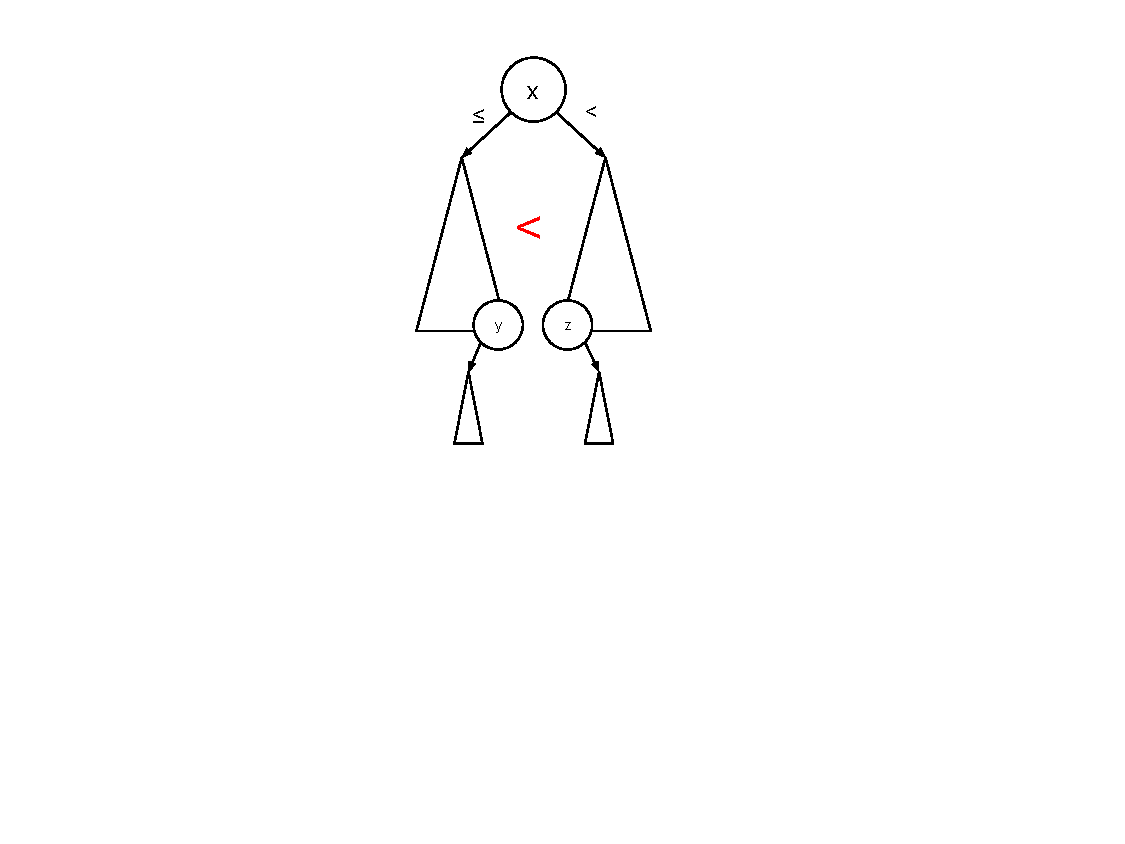
\includegraphics[width=14cm]{images/tree_delete_1}
  
  \end{frame}
  
    
  \begin{frame}[fragile]
  \frametitle{Изтриване}
  
  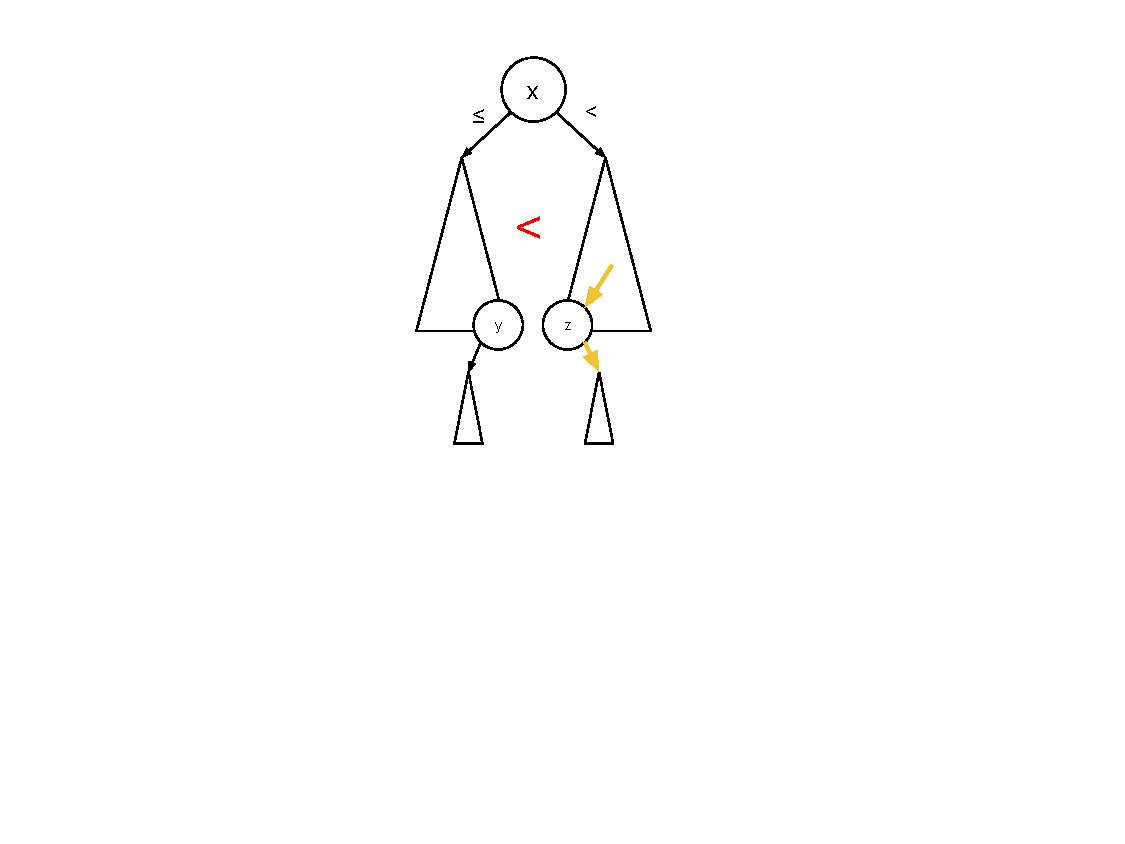
\includegraphics[width=14cm]{images/tree_delete_2}
  
  \end{frame}

  
  \begin{frame}[fragile]
  \frametitle{Изтриване}
  
  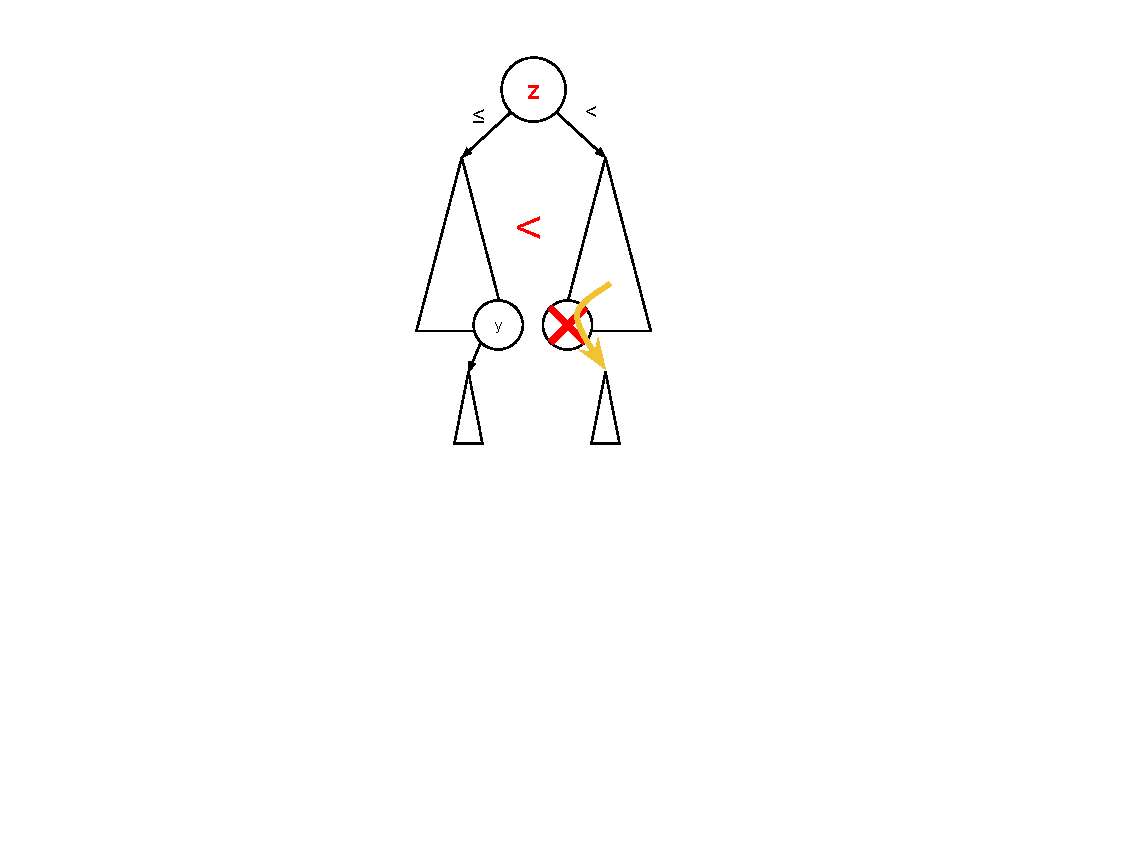
\includegraphics[width=14cm]{images/tree_delete_3}
  
  \end{frame}
  



\begin{frame}
  \centerline{Благодаря за вниманието!}
\end{frame}


\end{document}


\begin{columns}[t]
  \begin{column}{0.3\textwidth}

  \end{column}
  \begin{column}{0.7\textwidth}

  \end{column}
\end{columns}


